\documentclass[11pt,a4paper]{scrartcl} %scrartcl from KOMA-script uses sans headers and looks less latexy than article
%\usepackage[doublespacing]{setspace}
%\usepackage[capposition=top]{floatrow} %for notes under pics
%\usepackage[nomarkers]{endfloat}
\usepackage{natbib}
\usepackage[utf8]{inputenc}
%\usepackage{amsmath}
%\usepackage{amsfonts}
%\usepackage{amssymb}
\usepackage[left=2.5cm,right=2.5cm,top=3cm,bottom=3cm]{geometry}
\usepackage[pdftex, hidelinks]{hyperref}
\usepackage{graphicx}
\usepackage{booktabs}
\usepackage[blocks]{authblk} %for affil
\usepackage{url}
\usepackage{tabularx}
\usepackage{float} %allows the H positioning specifier
\usepackage{csvsimple}
\usepackage[nomessages]{fp}
\usepackage{xcolor}
\usepackage{enumitem}
\setlist{noitemsep} % \setlist{nosep} to reove separation around lists as well


%citation cheat sheet:
	%\ cite{key}				Jones et al. (1990)
	% \citet{key1,key2}			Jones et al. (1990); Ladze (1986)
	% \citet{key}				Jones et al. (1990)
	% \citet*{key}				Jones, Baker, and Smith (1990)
	% \citep{key}				(Jones et al. 1990)
	% \citep{key1,key2}			(Jones et al. 1990; Ladze 1986)
	% \citep*{key}				(Jones, Baker, and Smith 1990)
	% \citep[p.~99]{key}		(Jones et al., 1990, p. 99)
	% \citep[e.g.][]{key}		(e.g. Jones et al., 1990)
	% \citep[e.g.][p.~99]{key}	(e.g. Jones et al., 1990, p. 99)
	% \citeauthor{key}			Jones et al.
	% \citeauthor*{key}			Jones, Baker, and Smith
	% \citeyear{key}			1990
	% \citealt{key} 			Jones et al. 1990


\newcommand{\figureloc}{C:/Users/Koen/Dropbox/PhD/Papers/CongoGBV/Figures}
\newcommand{\tableloc}{C:/Users/Koen/Dropbox/PhD/Papers/CongoGBV/Tables}
\newcommand{\bibloc}{C:/Users/Koen/Dropbox/Literatuur/Mendeley/Bibtex/CongoGBV}





\begin{document}

\author{Koen Leuveld}

\affil{Development Economics Group, Wageningen University \\
\href{mailto:koen.leuveld@wur.nl}{koen.leuveld@wur.nl}}



\title{Sexual Violence, conflict and intra-household relations}
\subtitle{Exploratory evidence from a list experiment in Eastern DR Congo} %needs scrartcl

\maketitle

\begin{center}
\textcolor{red}{\Large VERY EARLY DRAFT!!!!}
\end{center}
%\begin{abstract}
%Abstract to come
%\end{abstract}



%literature to add somewhere:
%\cite{Saile2013} investigate the correlates of Intimate Partner Violence for a sample of conflict-exposed women in Northern Uganda. They find that while the level of conflict exposure predicts physical violence, sexual violence is more associated with the level of childhood familial violence. This link between current and past experiences of violence suggests that the effect of conflict on violence is deeper than just the direct effect. People traumatized during the conflict (either because they were victims or perpetrators) are more likely to be victimized later on. CHECK OOK NOG DE REFERENTIES VOOR EEN DIEPERE ONDERBOUWING VAN DIT PUNT.

%\cite{Muller2019} investigate the link between the conflict in Gaza and Domestic Violence. They find that exposure to conflict increases the incidence of DV. A woman's bargaining position decreases the incidence. IN DE LIT LIJST MEER ARTIKELEN OVER IPV <-> VIOLENCE

%\cite{Boesten2018}: collection of papers with some qualitative blabla. Could be worthwhile.


%%%%%%%%%%%%%%%%%%%%%%%%%%
\section*{Introduction}
%%%%%%%%%%%%%%%%%%%%%%%%%

\paragraph{}
%Hook
The high incidence of Sexual and Gender Based Violence (SGBV) in the Congo has been a prominent area of attention for the international development community over the past decades. Often, this high incidence of SGBV has been linked to the various violent conflicts the country has seen since the 1990s. In the policy domain, attention for the link between conflict in general and SGBV increased at the end of 1990s, when rape was used strategically by armed actors during armed conflicts in Rwanda and Bosnia  \citep{Kirby2015}. In Congo in particular, the issue has been on the agenda since 2002 when the NGO Human Rights Watch published a report on the topic \citep{HRW2002}. Since then, the issue has received attention by the UN, governments, NGOs and even celebrities \citep{Baaz2013}. This attention is understandable, as even outside of conflict settings, the psychological, social and economic costs of SGBV are staggering \citep{Post2002,Peterson2018}. To use this a weapon defies the imagination of Western audiences. Consequently, Congo to nearly become synonymous with rape, even called the ``rape capital of the world''. Tremendous international efforts have been made to implement or support projects to assist the victims of SGBV. The 2018 Nobel Peace prize was awarded to Dr. Denis Mukwege, for his work on victims of SGBV at Bukavu's Panzi Hospital.
 
\paragraph{}
%research question
To adequately address this issue, data on the victims of SGBV is of crucial importance. In this paper, I explore the characteristics of the victims SGBV to uncover the dynamics and potential drivers of SGBV.In particular, I consider conflict victimization, intra-household dynamics, and poverty as potential characteristics.

\paragraph{}
%Antecedents

%Add papers:
%Kelly2018: finds that IPV increased in districts that experienced conflict in Liberia. 

While estimates for the incidence of SGBV in DR Congo vary, they are invariably high: ranging from 15\% to 40\% \citep{Johnson2010,Peterman2011}. The conflict that has persisted in the country for the past decades has been frequently cited as the most important driver of SGBV. This is particularly true for policy circles, where the framing of SGBV in Congo as ``weapon of war'' is popular \citep{Baaz2013,Kirby2015}. There is empirical evidence that backs up this framing. \cite{Johnson2010} carried out a large-scale survey in Eastern DRC to investigate incidence and perpetrators of GBV. They find that the majority of sexual violence reported by their respondents was conflict-related; of female victims of sexual violence, 74.3\% reported being victim to conflict-related sexual violence. It is therefore not surprising that the topic of GBV in Congo has often been analysed within the context of violence \citep{Baaz2013}. Likewise, the aspect of the conflict that has received the most world-wide media attention has been GBV \citep{Autesserre2012a}.  
%Bouta, T., G. Frerks, and I. Bannon (2005) Gender, Conflict and Development. The World Bank, Washington, DC
\paragraph{}
This view of the central role of conflict in sexual violence has come under increasing scrutiny. It has been argued that this focus on the relationship between sexual violence and conflict has been counter-productive, as it has distracted attention from other pressing problems the country faces \citep{Autesserre2012a, Hilhorst2018,Porter2019}. Moreover, it risks missing the civilian perpetrators of SGBV, which are at least equally important as perpetrators from armed groups. There is empirical evidence for this position too. Based on DHS data, \cite{Peterman2011} find that Intimate Partner Violence is a large contributor to the incidence of sexual violence in Congo. \cite{Hilhorst2018} argues that the local NGO community in Eastern Congo is well aware of this, and uses the increased funds related to the massive attention generated by the ``weapon of war'' account of SGBV in Congo to fund projects to improve female empowerment in Congo and in this way prevent SGBV.  However, there is a long way to go, and women still hold a precarious position in Congolese society. For example, views that men have the right to physically abuse their wife if she is disobedient are broadly held \citep{Quattrochi2019}.
%Tia Palermo and Amber Peterman, ‘Undercounting, overcounting and the longevity of flawed estimates: statistics on sexual violence in conflict’, Bulletin of the World Health Organization, no. 89, 2011, pp. 924–5;
\paragraph{}
A large problem underlying the analysis of drivers and dynamics of SGBV is the paucity of reliable data. This exacerbated by the fact that the empirical studies that do exist, contradict each other. While one study finds conflict-related perpetrators are responsible for the majority of cases of SGBV \citep{Johnson2010}, another finds intimate partners as the most common culprits \citep{Peterman2011}. \citet{Stark2017} provide a possible explanation for this discrepancy. In a study where 87 women and girls in South Kivu were interviewed using Audio Assisted Self-Interviews (ACASI) techniques,they find that 14\% of respondents reported having been victim of sexual coercion. Half of these were perpetrated by the respondents' husbands or boyfriends. Crucially, in complementary group discussions, respondents did not bring up intimate partners at all. This points at the difficulties of collecting accurate data about GBV, and the importance of data collection methodologies. 

\paragraph{}
%Contribution
This paper contributes to the empirical evidence base on the incidence of GBV in Eastern Congo by using a list experiment to obtain reliable estimates of the incidence of SGBV. List experiments remove the bias in answering sensitive question, by removing the possibility of the researcher (or anyone else) to view individual answers to the sensitive topic. However, group-level analysis is still possible, to provide estimates of correlates of GBV. Combined with rich data from a household survey and behavioural experiments, collected in 2012 and 2014, this approach allows for a rich characterization of victims of GBV. As such a characterization is lacking thusfar, this data can be of tremendous usefulness in addressing and preventing GBV.
%perhaps note that tia finds no predictors for GBV.

\paragraph{}
%Road Map
I find no correlation between victimization of GBV and victimization of the conflict. I do find a strong correlation between victimization of GBV and intra-household dynamics: the result from a bargaining game, and the pre-marriage relative status of the wife and husband. This early draft of the paper is structured as follows: first I describe the research setting and data. I then present the results from various analyses on the list experiments conducted. In the concluding remarks, I contextualize the findings and present policy implications.

%%%%%%%%%%%%%%%%%%%%%%%%%%%%%%%%
\section*{Background and data}
%%%%%%%%%%%%%%%%%%%%%%%%%%%%%%%%
\paragraph{}
%to do in this section:
%add map.
%answer data questions
%add distributions of balls
\subsection*{Background}
The main source of data for this study is a household survey that was undertaken in 2014 as part of the evaluation of Dutch development aid in Eastern Congo. This evaluation concerned projects ran by four NGOs in the territories of Kabare, Fizi and Uvira, and the commune of Bagira, all in South Kivu province. Each individual project was small, and unlikely to have affected rates across the whole sample. The household questionnaire contained a final module that: (i) collected detailed information on gender attitudes; (ii) contained a list experiment designed to elicit the incidence of SGBV among female respondents; and (iii) contained a risk bargaining game. 

\begin{table}[htbp]
	\centering
	\caption{Gender module sample make up}
	\label{tab:bargsample}
	\begin{tabular}{l c c c c c}
		\toprule
		& \multicolumn{5}{c}{Husband} \\
Wife&Consented&Refused&Absent&No Husband&Total \\
\hline
Consented&184&3&253&153&593 \\
Refused&0&0&0&1&1 \\
Absent&4&0&0&1&5 \\
No Wife&282&3&2&3&290 \\
Total&470&6&255&158&889 \\
		\bottomrule
	\end{tabular}
\end{table}

\paragraph{}
Where possible, this gender module was administered to a both the head of the household and the spouse of the household head (in the vast majority of the cases, the husband is considered the head, but it was left open to the respondent to indicate the head). Table \ref{tab:bargsample} displays how the sample is built up. In total, there were 889 respondents to the survey. In 593 household, the wife of the household head (or the single female head, for convenience I will refer to both as wife) consented to responding to the gender module. In 1 household, the wife refused; in 5, the wife was absent during the interview, and in 290 households the head of the household had no wife. In 470 households, the husbands consented to the module, 6 refused, 255 husbands were absent, and in 158 households the head of the household was an unmarried woman. For 184 households, we have both husband and wife responding to the module. Efforts to increase this number, by tracking down absent household heads, were constricted by the limited time field teams had in each community, due to the security situation at the time of field work. \textcolor{red}{HOW DOES THIS AFFECT MY ESTIMATES, AND HOW CAN I MITIGATE THIS?}

\subsection*{List Experiment}
\paragraph{}
%what are they?
A major concern in collecting data on SGBV is reporting bias.Respondents are unlikely to be comfortable to truthfully answer questions about SGBV. What's worse, this unwillingness may be correlated to the identity of the perpetrators\citep{Stark2017}. Using answers to direct questions would thus lead to an underestimate of the incidence of SGBV, and biased estimates for the correlates of SGBV, due to the non-random nature of non-response. List Experiments have gained popularity in recent years as a way of address this issue by not asking the sensitive question directly. Instead, respondents are presented with a list of issues and indicate the number of issues from the list they have faced. By adding the sensitive item to the list of issues for half of the respondents (randomly selected), estimates for incidence of the sensitive item can be obtained by comparing the mean number of issues faced in both groups (hence ``item count technique'' as an alternative name for List Experiments). The advantage is thus that answers are guaranteed to be anonymous: the interviewer (or the data analyst) does not know the number of non-sensitive issues the respondent faces and so has no way of knowing the answer to sensitive item. This anonymity removes the need to hide the answer. 


\paragraph{}
%examples:
%\cite{Chuang2019} find that LEs weren't very precise.

This approach has been applied to a wide range of topics, such as sensitve political opionions \citep{Frye2017,Blair2014,Meng2017} and SGBV \citep{Bulte2019}. \cite{Bulte2019} is of particular interest to the current paper. They compare the results of direct questioning and list experiment to assess the incidence of IPV among beneficiaries of a program to boost female empowerment in Vietnam. They find that using direct questioning yields underestimates of the incidence of IPV. Moreover, the treatment effect of the project reverses its sign when using the List Experiment, compared to using direct questioning. This underlines the potential of List Experiments to address potential biases caused by reporting bias and direct questions.

%hoe ziet mijn implementatie er uit/
For the list experiment, the female respondents were randomly divided into two groups. This was done by the electroninc survey software (ODK), based on the randomly assigned ID codes. I follow \cite{Imai2011} in calling these groups Treatment and Control. The groups were told by the interviewer; ``I will read 4 (or 5) problems that women can experience. These can be sensitive problems. When you've experienced a problem \textbf{in the last year}, please drop one of the balls to the ground. I will not look at when you drop these balls, and only want to know the total number of balls at the end.'' The first group (Control) was presented with the following issues:
\begin{itemize}
	\item Lack of food;
	\item Lack of money;
	\item Theft; and,
	\item Sterility. %sell dit, mensen kunnen hier moeite mee hebben. Is er een manier om te checken? zeker! check \cite{Chuang2019}!
\end{itemize}

\paragraph{}
Women in the second group (Treatment) were presented with the same four items, but a fifth item was added: Sexual Violence. After all items were read, the interviewer asked the respondent to count the number of balls, and report the number. The questionnaire was field tested prior to field work to ensure that respondents understood these concepts. All interviewers were thoroughly trained in the protocols, and the electronic questionnaire was programmed in such a way to ensure compliance to the protocol.

%hoe doe ik de analyse, en interpreteer ik coefficienten etc.
While the indirect nature of List Experiments prevents reporting bias, this does come at a cost of efficiency in statistical analysis. The incidence is easily computed by subtracting the mean of issues faced in the control group from the mean number of issues in the treatment group. This means that sample sizes have to be far larger for List Experiments than for direct questions. In a regression framework, the incidence would be estimated as follows:

\begin{equation}
\label{eq:basic}
NumIssues_i = \beta_0 + \beta_1 Treatment_i + \epsilon_i
\end{equation}

Where \(NumIssues_i\) is the number of issues faced by repsondent i, and \(Treatment_i\) is her treatment assignment. Coefficient \(\beta_1\) yields the estimate for the incidence. To find correlates of SGBV, equation \ref{eq:basic} can be augmented using interaction terms as follows: 
\begin{equation}
\label{eq:interaction}
NumIssues_i = \beta_0 + \beta_1 Treatment_i + \beta_2 X_i + \beta_3 Treatment_i X_i + \epsilon_i
\end{equation}

Where \(X_i\) is an explanatory variable and coefficient \(\beta_3\) gives the estimate for the additional incidence of SGBV associated with a unit increase of \(X\). This can be easily modified to allow for more variables. Again, this is much less efficient than when using direct questioning. By using more sophisticated methods proposed by \citet{Imai2011} (and implemented by \cite{Tsai2019} in Stata), more efficient estimates can be obtained. 


\subsection*{Bargaining}
 \paragraph{}
 The risk bargaining game in the module was modified from \cite{Martinsson2009}. In the game, couples choose between a set of six risky lotteries, based on \cite{Eckel2002}. The lotteries presented range from fairly low-risk ones -- where low and high pay-out are nearly equal -- to high-risk one -- where there is a large difference between high and low pay-outs (see Table \ref{tab:bargaining} for details of the lotteries). The respondents first choose individually (without knowing their partner's choice), and then jointly. By comparing the couple decision with the individual decision, I obtain an indicator for bargaining power. The difference between the procedure used by \cite{Martinsson2009} and the one here, is that they use a risk experiment based on \cite{Holt2002}. However, this is a more complicated experiment compared to \citeauthor{Eckel2002}. This added complication may cause participants to not fully understand the procedure, leading to poor results \citep{Dave2010a}. Given the low numeracy of the subjects, I implemented the simpler of the two experiments.

\begin{table}
	\centering
	\caption{Bargaining game lotteries}
	\label{tab:bargaining}
	\begin{tabular}{l c c c c}
	\toprule
	\# & Low & High & Expected & Risk aversion \\
	\hline
	1 & 4,000 CDF & 4,000 CDF & 4,000 CDF & Extremely risk-averse \\
	2 & 3,600 CDF & 4,800 CDF & 4,200 CDF & Extremely risk-averse \\
	3 & 3,200 CDF & 5,600 CDF & 4,400 CDF & Moderately risk-averse \\
	4 & 2,800 CDF & 6,400 CDF & 4,600 CDF & Moderately risk-averse \\
	5 & 2,400 CDF & 7,200 CDF & 4,800 CDF & Risk-neutral \\
	6 & 1,400 CDF & 8,200 CDF & 4,800 CDF & Risk-loving \\ 
	\bottomrule
	\end{tabular}
\end{table}

\subsection*{Conflict}
\paragraph{}
Conflict victimization data was not collected during the 2014 round of the survey. However, for 479, conflict data is available from the 2012 round of data collection. Since the majority of conflict events happened before this time, I used this data as a proxy for conflict exposure. This allows for the historic effects of conflict. I used ACLED data for current effects.

%EXPAND



\subsection*{Descriptive Statistics}
\paragraph{}
Table \ref{tab:balance} presents descriptive statistics of the sample. The household questionnaire contained detailed questions about the marriage of the household head. One question asked was whether the family of the wife or the husband had more land at the time of marriage. In consultation with local partners (including NGOs and universities) this was chosen as the best proxy for status, due to the importance of agriculture in the area. In 38\% of the cases, the husband's family had more land, in 24\% of the cases the wife's family did. Note that only 384 households responded to this question, as some refused to give a definite answer. As for the bargaining game: in 40\% of the cases, the couple's bargained decision was closest to the husbands. In 27\% of the cases, the couple's decision was closest to the wife's. In the remainder, the final decision was equally close to both. Conflict victimization is high in the sample. 80\% of the household indicate having lost property due to the conflict; 53\% report having lost a family or household member. The women in the sample, on average, contribute 20\% of the cash income in their household, and 24\% of the in-kind income. About 61\% of the households have a tin roof (with the vast majority of the remainder owning simple thatch roofs), and 49\% own any kind of livestock.

\paragraph{}
%is hh_id 1 determined randomly? If not, perhaps exlude it?
The treatment and control group are not perfectly balanced across some of the variables presented in table \ref{tab:balance} (Column 7). As randomization was done at the time of data collection (based on randomly assigned ID codes). An F-test on the differences between treatment and control being jointly equal to zero fails to reject the null-hypothesis that they are equal (p=0.20). However, care should be taken in interpreting the differences in the variables with differences: results being closer to the women's choice, and the cash income of the household. 

\begin{table}[hp] \centering
\newcolumntype{C}{>{\centering\arraybackslash}X}

\caption{Descriptive statistics by treatment assignemt}
\label{tab:balance}
{\footnotesize
\begin{tabularx}{\linewidth}{lCCCCCCC}

\toprule
&{(1)}&{(2)}&{(3)}&{(4)}&{(5)}&{(6)}&{(7)} \tabularnewline
&\multicolumn{2}{c}{All}&\multicolumn{2}{c}{Treatment}&\multicolumn{2}{c}{Control}&{(4)-(6)}\tabularnewline \midrule
{}&{N}&{Mean}&{N}&{Mean}&{N}&{Mean}&{ } \tabularnewline
\midrule \addlinespace[\belowrulesep]
Number of reported issues&593&2.49&291&2.65&302&2.34&0.30*** \tabularnewline
&&(0.94)&&(1.03)&&(0.83)& \tabularnewline
Conflict pre-2012: property lost&530&0.77&264&0.79&266&0.75&0.04 \tabularnewline
&&(0.42)&&(0.41)&&(0.43)& \tabularnewline
Conflict pre-2012: HH member killed&530&0.49&264&0.51&266&0.48&0.03 \tabularnewline
&&(0.50)&&(0.50)&&(0.50)& \tabularnewline
Conflict 2013--2014: Viol. against civilians&496&6.73&239&6.68&257&6.77&--0.08 \tabularnewline
&&(4.69)&&(4.70)&&(4.69)& \tabularnewline
Family MR had more land&450&0.33&224&0.33&226&0.33&--0.00 \tabularnewline
&&(0.47)&&(0.47)&&(0.47)& \tabularnewline
Family FR had more land&450&0.21&224&0.22&226&0.19&0.02 \tabularnewline
&&(0.41)&&(0.41)&&(0.40)& \tabularnewline
Bargaining: choice Female Respondent&593&3.58&291&3.59&302&3.56&0.04 \tabularnewline
&&(2.06)&&(2.08)&&(2.05)& \tabularnewline
Barganing: choice Male Respondent&184&3.45&97&3.49&87&3.40&0.09 \tabularnewline
&&(2.14)&&(2.12)&&(2.18)& \tabularnewline
Bargaining: closer to MR&184&0.40&97&0.37&87&0.44&--0.07 \tabularnewline
&&(0.49)&&(0.49)&&(0.50)& \tabularnewline
Bargaining: closer to FR&184&0.27&97&0.32&87&0.21&0.11* \tabularnewline
&&(0.44)&&(0.47)&&(0.41)& \tabularnewline
Age of FR&593&41.09&291&40.49&302&41.67&--1.17 \tabularnewline
&&(14.01)&&(14.06)&&(13.96)& \tabularnewline
Age of MR&449&45.67&224&44.48&225&46.85&--2.37** \tabularnewline
&&(13.80)&&(13.09)&&(14.40)& \tabularnewline
HH Head Female&593&0.26&291&0.24&302&0.27&--0.03 \tabularnewline
&&(0.44)&&(0.43)&&(0.45)& \tabularnewline
FR completed primary education&593&0.25&291&0.26&302&0.25&0.01 \tabularnewline
&&(0.44)&&(0.44)&&(0.43)& \tabularnewline
FR completed secondary education&593&0.03&291&0.02&302&0.04&--0.02 \tabularnewline
&&(0.17)&&(0.13)&&(0.20)& \tabularnewline
MR completed primary education&449&0.63&224&0.63&225&0.63&0.01 \tabularnewline
&&(0.48)&&(0.48)&&(0.48)& \tabularnewline
MR completed secondary education&449&0.20&224&0.19&225&0.20&--0.01 \tabularnewline
&&(0.40)&&(0.39)&&(0.40)& \tabularnewline
Household has a tin roof&593&0.61&291&0.62&302&0.59&0.03 \tabularnewline
&&(0.49)&&(0.49)&&(0.49)& \tabularnewline
Household owns livestock&593&0.49&291&0.51&302&0.47&0.03 \tabularnewline
&&(0.50)&&(0.50)&&(0.50)& \tabularnewline
territory==Uvira&593&0.24&291&0.24&302&0.23&0.01 \tabularnewline
&&(0.43)&&(0.43)&&(0.42)& \tabularnewline
territory==Fizi&593&0.63&291&0.65&302&0.62&0.03 \tabularnewline
&&(0.48)&&(0.48)&&(0.49)& \tabularnewline
Project Beneficary&593&0.50&291&0.49&302&0.50&--0.01 \tabularnewline
&&(0.50)&&(0.50)&&(0.50)& \tabularnewline
\bottomrule \addlinespace[\belowrulesep]

\end{tabularx}
\begin{flushleft}
\footnotesize FR = Female Respondent; MR = Male Respondent; Standard Deviations in parentheses; *p $<$ 0.1,**p $<$ 0.05,***p $<$ 0.01
\end{flushleft}
}
\end{table}


%some examples on how to interpret list experiments:
%\cite{Meng2017} run various types of models. Consistently refer to mean difference models, and Maximum Likelihood models

%\cite{Blair2014}: extremely detailed stuff. Thread carefully!
%\cite{Frye2017} simple difference in means model.

%%%%%%%%%%%%%%%%%%%%%%%%%%%%%%%%
\section*{Results}
%%%%%%%%%%%%%%%%%%%%%%%%%%%%%%%%
\textcolor{red}{NB: THIS SECTION IS WRITTEN SO THAT COEFFICIENTS AND ESTIMATES ARE PULLED FROM EXTERNAL FILES AUTOMATICALLY. THE TEXT IS THUS VERY GENERIC. WILL UPDATE ONCE EVERYTHING IS MORE FINAL}
%command to get incidences from csv file
\newcommand{\incid}[2]{\csvreader[filter strcmp={\key}{#1}]{\tableloc/incidence.csv}{key=\key,#2=\inc}{\inc}}

\paragraph{}
First, I compare the number of issues faced by the Treatment and Control groups in the entire sample. I then compare the number of issues faced in several sub-groups. These sub-groups divide the sample along dimensions of intra-household dynamics, conflict exposure and asset holdings. In the full sample, the difference between the group who were presented with only four issues (the control group) and the group who were presented four issues plus GBV (the treatment group) is the estimate of the incidence of GBV. The average number of issues reported by the control group is \incid{overall1}{mean0}, while the number if issues reported by the treatment group is \incid{overall1}{mean1} (see Figure \ref{fig:meancompare_overall}). The difference of \incid{overall1}{incidence} implies that the incidence of GBV is \incid{overall1}{incidence_pct}\% in this sample. The p-value for a t-test on this difference is \incid{overall1}{p}. This estimate is roughly in line with previous estimates \citep{Peterson2018,Stark2017,Johnson2010}.

\begin{figure}[H]
  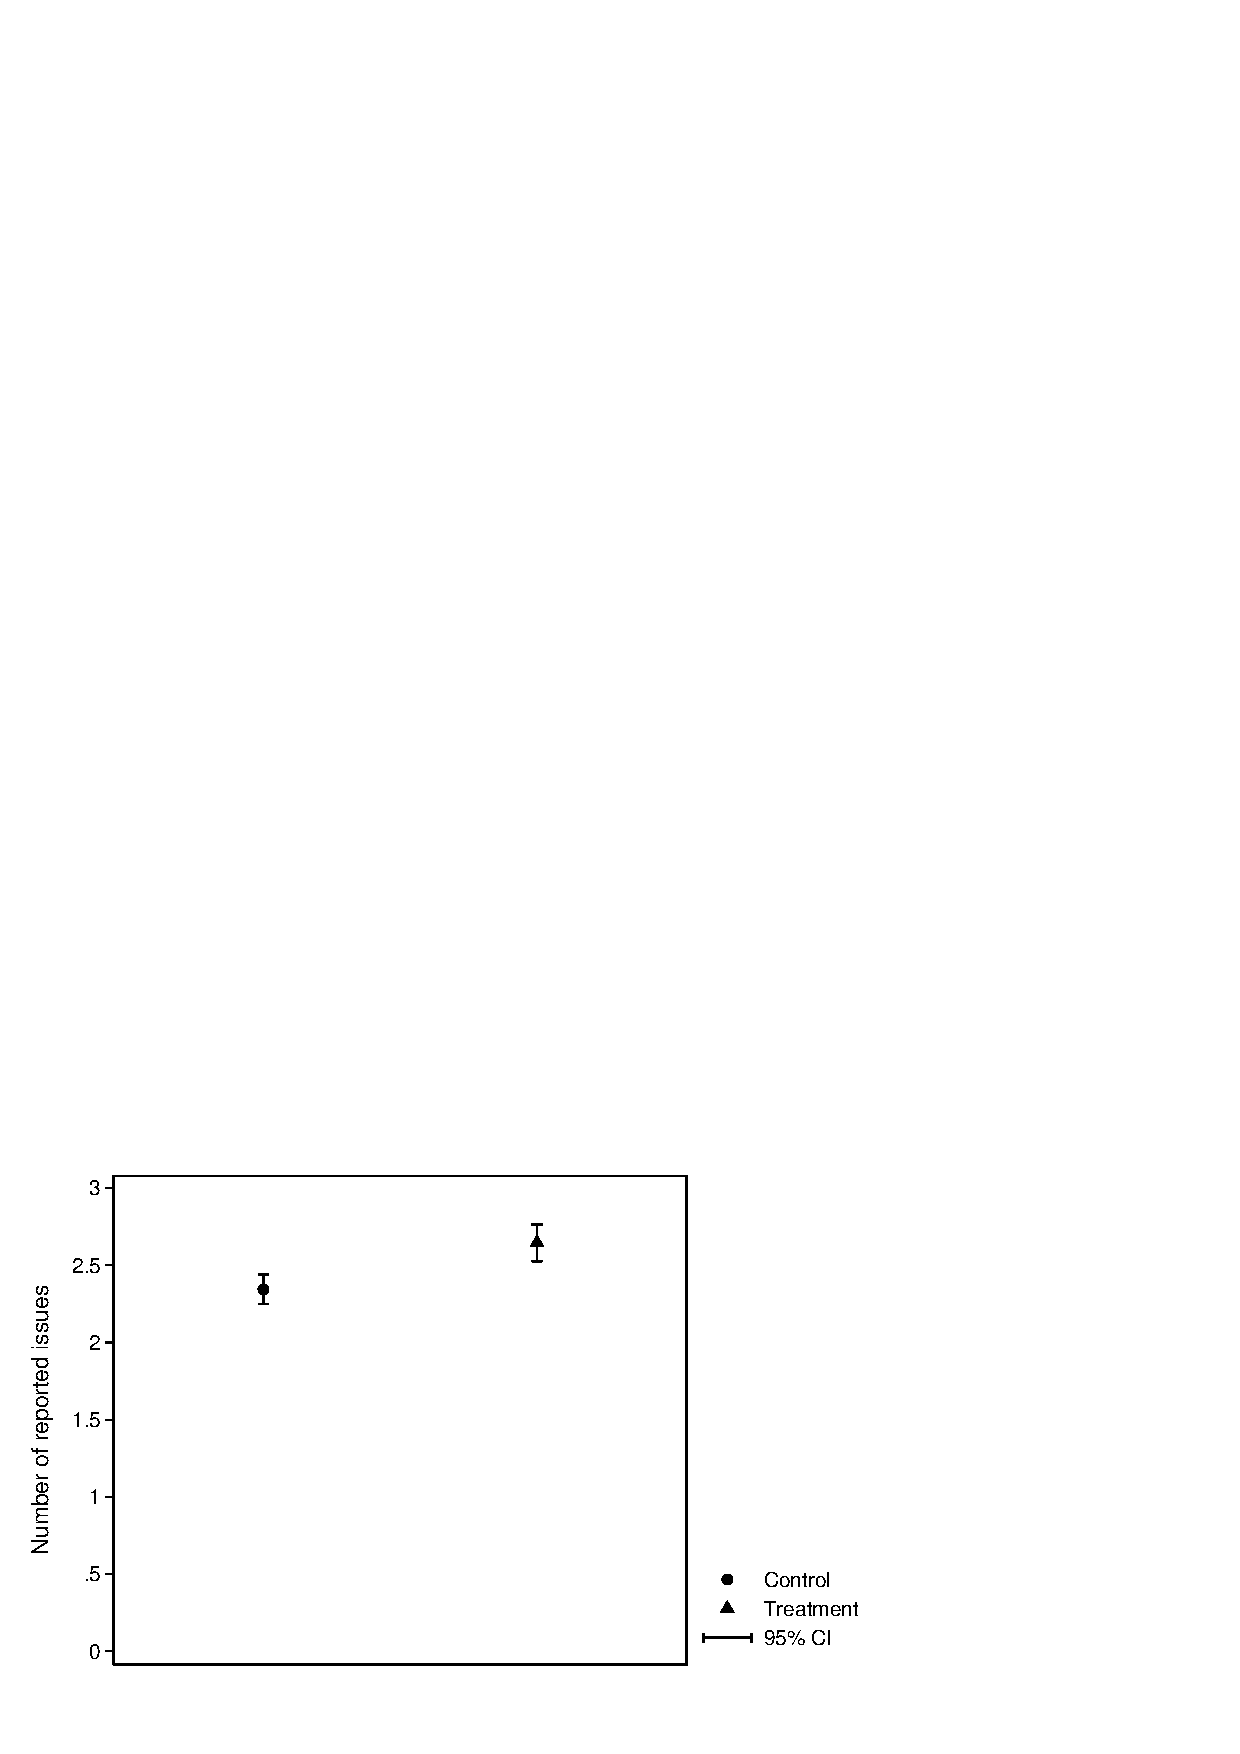
\includegraphics[width=0.6\linewidth]{\figureloc/meancompare_overall.png}
  \caption{Comparison of means of issues faced: treatment vs. control.}
  \label{fig:meancompare_overall}
\end{figure}

\subsection*{Intra-household Dynamics}

\paragraph{}
 The first dimension over which I create sub-groups is intra-household dynamics. First, I compare women across the relative status of the partners at the time of marriage. For this, I use the land held by the partners' families at the time of marriage as proxy for status (Figure \ref{fig:meancompare_mar1}). In the group where the wife had more status before the marriage (n=\incid{statpar1}{n}), the average number of issues was \incid{statpar1}{mean0} for the control group, and \incid{statpar1}{mean1} for the treatment group. The difference in means implies a rate of GBV of \incid{statpar1}{incidence_pct}\% (p-value of a t-test on the means = \incid{statpar1}{p}). In the group where the partners were of equal standing (n=\incid{statpar2}{n}), the average number of issues was \incid{statpar2}{mean0} for the control group, and \incid{statpar2}{mean1} for the treatment group. This implies a rate of GBV of \incid{statpar2}{incidence_pct} (p = \incid{statpar2}{p}). In the group where the husband had more status (n=\incid{statpar3}{n}), the average number of issues was \incid{statpar3}{mean0} for the control group, and \incid{statpar3}{mean1} for the treatment group. This implies a rate of GBV of \incid{statpar3}{incidence_pct} (p = \incid{statpar3}{p}).

\begin{figure}[H]
  \includegraphics[width=0.6\linewidth]{\figureloc/meancompare_mar1.png}
  \caption{Comparison of means of issues faced by pre-marriage status.}
  \label{fig:meancompare_mar1}
\end{figure}

\paragraph{}
The second intra-household aspect I explore is derived from the results of a bargaining game played with couples. Couples first took a decision individually, and then jointly. I then create three groups, based on whether the joint decision is closer to the husband's decision, to the wife's, or if the distance is equal. See figure \ref{fig:meancompare_mar2}. In the group where the couple decision was closest to the wife's decision (n=\incid{bargresult1}{n}), the average number of issues was \incid{bargresult1}{mean0} for the control group, and \incid{bargresult1}{mean1} for the treatment group. This implies a rate of GBV of \incid{bargresult1}{incidence_pct}\% (p = \incid{bargresult1}{p}). In the group where the couple decision was equally close to the husband and wife (n=\incid{bargresult2}{n}), the average number of issues was \incid{bargresult2}{mean0} for the control group, and \incid{bargresult2}{mean1} for the treatment group. This implies a rate of GBV of \incid{bargresult2}{incidence_pct}\% (p = \incid{bargresult2}{p}). In the group where the couple decision was closest to the husband's (n=\incid{bargresult3}{n}), the average number of issues was \incid{bargresult3}{mean0} for the control group, and \incid{bargresult3}{mean1} for the treatment group. This implies a rate of GBV of \incid{bargresult3}{incidence_pct}\% (p = \incid{bargresult3}{p}).

\begin{figure}[H]
  \includegraphics[width=0.6\linewidth]{\figureloc/meancompare_mar2.png}
  \caption{Comparison of means of issues faced by bargaining result.}
  \label{fig:meancompare_mar2}
\end{figure}

\paragraph{}
The final intra-household variable I use to compare women, is their relative contribution to the household's cash income (see figure \ref{fig:meancompare_mar3}). The household questionnaire collected data on all activities of household members, and what the contribution of these activities were to household income. I sum this for all activities for the women in the sample, and compare those who contribute more than 50\% of cash income with those who do not. In the group where the woman does not contribute more than 50\% of cash income (n=\incid{contribcashyn0}{n}), the average number of issues was \incid{contribcashyn0}{mean0} for the control group, and \incid{contribcashyn0}{mean1} for the treatment group. This implies a rate of GBV of \incid{contribcashyn0}{incidence_pct}\% (p = \incid{contribcashyn0}{p}). In the group where the woman does contribute more than 50\% of cash income (n=\incid{contribcashyn1}{n}), the average number of issues was \incid{contribcashyn1}{mean0} for the control group, and \incid{contribcashyn1}{mean1} for the treatment group. This implies a rate of GBV of \incid{contribcashyn1}{incidence_pct}\% (p = \incid{contribcashyn1}{p}). 

\begin{figure}[H]
  \includegraphics[width=0.6\linewidth]{\figureloc/meancompare_mar3.png}
  \caption{Comparison of means of issues faced across contribution to cash income.}
  \label{fig:meancompare_mar3}
\end{figure}


\paragraph{}
In order to test whether the differences in incidence between the subgroups created by each variable above, I estimate the model of equation \ref{eq:interaction} above, each time using a different variable as $X$. I plot the coefficients, as well as their 95\% confidence intervals in figure \ref{fig:regfig_mar}. Note that each coefficient is a separate model. I find that women whose families had more land than their husband's families face are victimized by SGBV at a significantly lower rate than other women. I find the same for women who have a better bargaining position, as indicated by the bargaining game.

\begin{figure}[H]
  \includegraphics[width=0.6\linewidth]{\figureloc/regfig_mar.png}
  \caption{Regression coefficients.}
  \label{fig:regfig_mar}
\end{figure}

\subsection*{Conflict}
I then compare the conflict history of the respondents' households, to assess whether conflict victimization correlates with the incidence of GBV. I use data collected from an earlier round of the study that collected detailed conflict exposure data. First, I compare respondents who live in households who have suffered loss of (or damage to) property, including agricultural fields, due to conflict. See \ref{fig:meancompare_conf1}. In the non-victimized group (n=\incid{victimproplost0}{n}), the average number of issues was \incid{victimproplost0}{mean0} for the control group, and \incid{victimproplost0}{mean1} for the treatment group. This implies a rate of GBV of \incid{victimproplost0}{incidence_pct}\% (p = \incid{victimproplost0}{p}). For the group that has suffered loss of property due to the conflict (n=\incid{victimproplost1}{n}), the average number of issues was \incid{victimproplost1}{mean0} for the control group, and \incid{victimproplost1}{mean1} for the treatment group. This implies a rate of GBV of \incid{victimproplost1}{incidence_pct}\% (p = \incid{victimproplost1}{p}).

\begin{figure}[H]
  \includegraphics[width=0.6\linewidth]{\figureloc/meancompare_conf1.png}
  \caption{Comparison of means of issues faced across conflict exposure.}
  \label{fig:meancompare_conf1}
\end{figure}

The second conflict indicator I examine, is whether the respondent's household has lost any household members or family as a consequence of the conflict.See \ref{fig:meancompare_conf2}. In the non-victimized group (n=\incid{victimfamlost0}{n}), the average number of issues was \incid{victimfamlost0}{mean0} for the control group, and \incid{victimfamlost0}{mean1} for the treatment group. This implies a rate of GBV of \incid{victimfamlost0}{incidence_pct}\% (p = \incid{victimfamlost0}{p}). For the group that has suffered loss of property due to the conflict (n=\incid{victimfamlost1}{n}), the average number of issues was \incid{victimfamlost1}{mean0} for the control group, and \incid{victimfamlost1}{mean1} for the treatment group. This implies a rate of GBV of \incid{victimfamlost1}{incidence_pct}\% (p = \incid{victimfamlost1}{p}).

\begin{figure}[H]
  \includegraphics[width=0.6\linewidth]{\figureloc/meancompare_conf2.png}
  \caption{Comparison of means of issues faced across conflict exposure.}
  \label{fig:meancompare_conf2}
\end{figure}


The third conflict indicator I examine, is the number of cases of violence against civilians in a 30km radius in the past month. I split the sample in two, using the median as a cutoff point. See \ref{fig:meancompare_conf3}. In the non-victimized group (n=\incid{acledviolence30d0}{n}), the average number of issues was \incid{acledviolence30d0}{mean0} for the control group, and \incid{acledviolence30d0}{mean1} for the treatment group. This implies a rate of GBV of \incid{acledviolence30d0}{incidence_pct}\% (p = \incid{acledviolence30d0}{p}). For the group that has suffered loss of property due to the conflict (n=\incid{acledviolence30d1}{n}), the average number of issues was \incid{acledviolence30d1}{mean0} for the control group, and \incid{acledviolence30d1}{mean1} for the treatment group. This implies a rate of GBV of \incid{acledviolence30d1}{incidence_pct}\% (p = \incid{acledviolence30d1}{p}). Note that the results presented here are robust to using number of battles or number of fatalities rather than the instances of violence against civilians; using 5,10,15,20 or 25km as a radius, or using a continuous variable, rather than a binary variable.  

\begin{figure}[H]
  \includegraphics[width=0.6\linewidth]{\figureloc/meancompare_conf3.png}
  \caption{Comparison of means of issues faced across conflict exposure.}
  \label{fig:meancompare_conf3}
\end{figure}


\paragraph{}
As above, I statistically test the differences in the differences of means by inserting the variables examined above in equation \ref{eq:interaction}. The results are displayed in figure \ref{fig:regfig_conf}. None of the coefficients plotted are significant at the 95\% level.

\begin{figure}[H]
  \includegraphics[width=0.6\linewidth]{\figureloc/regfig_conf.png}
  \caption{Regression coefficients of conflict indicators.}
  \label{fig:regfig_conf}
\end{figure}


\subsection*{Assets}
I then explore the relationship between asset holdings and GBV. The first asset I consider, is having a tin roof (figure \ref{fig:meancompare_ses1}). These roofs are a substantial improvement over thatch roofs, but about half the sample doesn't own them. This makes for a simple, yet non-arbitrary, way to split the sample in richer and poorer households.   In the group without tin roofs (n=\incid{tinroof0}{n}), the average number of issues was \incid{tinroof0}{mean0} for the control group, and \incid{tinroof0}{mean1} for the treatment group. This implies a rate of GBV of \incid{tinroof0}{incidence_pct}\% (p = \incid{tinroof0}{p}). For the group with tin roofs (n=\incid{tinroof1}{n}), the average number of issues was \incid{tinroof1}{mean0} for the control group, and \incid{tinroof1}{mean1} for the treatment group. This implies a rate of GBV of \incid{tinroof1}{incidence_pct}\% (p = \incid{tinroof1}{p}).

\begin{figure}[H]
  \includegraphics[width=0.6\linewidth]{\figureloc/meancompare_ses1.png}
  \caption{Comparison of means of issues faced across asset holdings (tin roof).}
  \label{fig:meancompare_ses1}
\end{figure}

\paragraph{}
A second asset with important status implications for the household is livestock (see figure \ref{fig:meancompare_ses2}).  In the group without livestock (n=\incid{livestockany0}{n}), the average number of issues was \incid{livestockany0}{mean0} for the control group, and \incid{livestockany0}{mean1} for the treatment group. This implies a rate of GBV of \incid{livestockany0}{incidence_pct}\% (p = \incid{livestockany0}{p}). For the group with tin roofs (n=\incid{livestockany1}{n}), the average number of issues was \incid{livestockany1}{mean0} for the control group, and \incid{livestockany1}{mean1} for the treatment group. This implies a rate of GBV of \incid{livestockany1}{incidence_pct}\% (p = \incid{livestockany1}{p}).

\begin{figure}[H]
\includegraphics[width=0.6\linewidth]{\figureloc/meancompare_ses2.png}
  \caption{Comparison of means of issues faced across asset holdings (livestock).}
  \label{fig:meancompare_ses2}
\end{figure}


\paragraph{}
As above, I statistically test the differences in the differences of means by inserting the variables examined above in equation \ref{eq:interaction}. The results are displayed in figure \ref{fig:regfig_ses}. None of the coefficients plotted are significant at the 95\% level.

\begin{figure}[H]
  \includegraphics[width=0.6\linewidth]{\figureloc/regfig_ses.png}
  \caption{Regression coefficients of conflict indicators.}
  \label{fig:regfig_ses}
\end{figure}




\paragraph{}
In summary, I find that women who are in a disadvantageous position in their household, either because they are of lower status, or because they have less bargaining power, are more likely to have experienced GBV. The results with respect to conflict were ambiguous, and I find no suggestion that respondents in poorer household experience GBV at a higher rate than their peers in richer households. If anything, I find the opposite. There are two large caveats with these findings: (i) they are not causal; (ii) by running separate comparisons, any conclusions are at risk of missing variable bias. While the first one is hard to address using list experiments, it is possible to come to more rigorous estimates of effects than presented so far. 

\subsection*{Regression analysis}
\paragraph{}
In table \ref{tab:results_regression} I display the results of a number of regressions. These are linear regressions: the coefficients reported should be interpreted as the interaction between each variable and the treatment indicator: i.e. the marginal effects of each variable on the difference in number of reported issues between control and treatment. For brevity, the level effects of each variable on the total number of issues are omitted, as these coefficients are not of interest here. In the first column, I report the results of including only endline survey measures; in the second, I add baseline conflict indicators; in the third I include results from the bargaining game. Finally, I estimate a full model. I find that neither conflict exposure, nor household asset holdings are correlated to the incidence of GBV. Intra-household dynamics on the other hand, are strongly correlated to GBV. Nearly all the GBV happens to women who live in male dominated households. From this, we cannot conclude that it is the husbands who perpetrate the violence. It may be possible that both GBV, and choosing partners of high status, are both determined by the same factors. However, contrary to popular narratives, we find no evidence of correlation to conflict exposure.


\newcommand{\coeffget}[3]{\csvreader[filter=\equal{\reg}{#1} \and \equal{\var}{#2}]{\tableloc/regs.csv}{var=\var,reg=\reg,#3=\coeff}{\coeff}}
%TEST: \coeffget{l1}{Delta:husbmoreland}{coef}

\begin{table}
	\caption{Results}\label{tab:results_regression}
	\begin{center}
	{
\def\sym#1{\ifmmode^{#1}\else\(^{#1}\)\fi}
\begin{tabular}{l*{4}{c}}
\hline\hline
                    &\multicolumn{1}{c}{(1)}   &\multicolumn{1}{c}{(2)}   &\multicolumn{1}{c}{(3)}   &\multicolumn{1}{c}{(4)}   \\
\hline
Family MR had more land&       0.419** &               &               &       0.451*  \\
                    &     (0.204)   &               &               &     (0.240)   \\
[1em]
Conflict pre-2012: HH member killed&               &       0.409** &               &       0.374** \\
                    &               &     (0.182)   &               &     (0.179)   \\
[1em]
Conflict 2013-2014: Viol. against civilians&               &               &      0.0120   &      0.0147   \\
                    &               &               &    (0.0224)   &    (0.0230)   \\
[1em]
FR empowerment attitudes&               &               &               &    0.000101   \\
                    &               &               &               &    (0.0199)   \\
[1em]
Age of FR           &     0.00843   &     0.00684   &     0.00563   &      0.0110   \\
                    &    (0.0161)   &    (0.0182)   &    (0.0186)   &    (0.0207)   \\
[1em]
Age of MR           &     -0.0122   &    -0.00929   &    -0.00778   &     -0.0111   \\
                    &    (0.0149)   &    (0.0162)   &    (0.0174)   &    (0.0189)   \\
[1em]
HH Head Female      &     0.00951   &     -0.0766   &       0.257   &       0.421   \\
                    &     (0.445)   &     (0.525)   &     (0.318)   &     (0.410)   \\
[1em]
FR completed secondary education&      -1.111***&      -1.347***&      -1.034***&      -1.249***\\
                    &     (0.320)   &     (0.351)   &     (0.336)   &     (0.332)   \\
[1em]
MR completed primary education&     -0.0390   &     -0.0655   &      -0.193   &      -0.263   \\
                    &     (0.166)   &     (0.178)   &     (0.181)   &     (0.177)   \\
[1em]
Household has a tin roof&       0.292   &       0.279   &       0.184   &       0.214   \\
                    &     (0.203)   &     (0.221)   &     (0.234)   &     (0.233)   \\
[1em]
Household owns livestock&     -0.0455   &    -0.00342   &      -0.142   &      -0.193   \\
                    &     (0.160)   &     (0.181)   &     (0.177)   &     (0.186)   \\
[1em]
territory==Uvira    &       0.418   &       0.202   &       0.438   &       0.205   \\
                    &     (0.264)   &     (0.342)   &     (0.288)   &     (0.360)   \\
[1em]
territory==Fizi     &       0.511*  &       0.232   &       0.504*  &       0.191   \\
                    &     (0.292)   &     (0.365)   &     (0.302)   &     (0.379)   \\
[1em]
Project Beneficary  &      0.0542   &      0.0121   &      0.0382   &      0.0732   \\
                    &     (0.163)   &     (0.177)   &     (0.157)   &     (0.167)   \\
[1em]
Constant            &      -0.162   &    -0.00267   &    -0.00290   &      -0.111   \\
                    &     (0.483)   &     (0.506)   &     (0.491)   &     (0.614)   \\
\hline
Observations        &         449   &         402   &         379   &         350   \\
\hline\hline
\end{tabular}
}

	\end{center}
\end{table}


\section*{Conclusion}
%restate the topic and its importance.
This study provided evidence on the victims of SGBV in Congo. Prevalence of SGBV is high in Congo, but little is known about the victims. To obtain this evidence, I used a list experiment to prevent disclosure bias.This allows me to find correlates of SGBV. I complemented this with a household bargaining game, designed to elicit often unobserved intra-household dynamics.

\paragraph{} 
In contrast to popular frames that paint a picture of conflict being the largest determinant of sexual violence (and sexual violence the most important outcome of conflict), I find no relationship between conflict exposure and SGBV. I also find no evidence for a difference in incidence of SGBV between poorer and richer household. I do find that victims of sexual violence were married to men of higher status (pre-marriage), and had less bargaining power in the household.

\paragraph{} 
These findings correspond to previous literature suggesting that intimate partners are more likely perpetrators of SGBV than members of armed groups \citep[see e.g.][]{Peterman2011}. The implication is that an end to the conflict in Eastern Congo will not bring an end to the problems women face. To reduce the incidence of SGBV, strong efforts to promote female empowerment are needed.







%interpretatie voorbeelden:
%\cite{Meng2017} first simply present mean differences; they then present a maximum likelihood model. Based on this model, they predict mean differences and present this as their quantity of interest. They have replication files online.

%\cite{Imai2011}: himself admits that the coefficients of the maximum likelihood method are difficult to compare. He therefore generates predicted values of shares of people answering affirmitively to the sensitive item for two subgroups.

%\cite{Bulte2019}: how they do interpret.


%bibliography, this is needed for bibtex
\clearpage 
\bibliographystyle{chicago}
%path to .bib file (e.g. automatically exported by mendeley) exclude the file extension!
\bibliography{C:/Users/Koen/Dropbox/Literatuur/Mendeley/Bibtex/CongoGBV}

\end{document}
